\chapter{Background and Theory}
\label{chap:BackgroundAndTheory}
This chapter provides the main concepts and theories used in the thesis. First, the SEAS model is presented in \autoref{sec:Theory_SEAS}, followed by a discussion of the resulting differential algebraic equation (DAE) in \autoref{sec:Theory_DAE}. Further, explicit and implicit time-adaptive integration methods are provided in \autoref{sec:Theory_TimeIntegration} and finally a physically motivated definition of the timestep is introduced in \autoref{sec:Theory_PhysicalTimeStepping}.

\section{Sequences of Earthquake and Aseismic Slip (SEAS)}
\label{sec:Theory_SEAS}
Two tectonic plates are separated by a zone of cracked and loose rocks, which are most likely to yield first under high stress \cite{introductionGeophysics}. In the SEAS model described by Rice \cite{GeneralSEASSimulations}, this zone is approximated by a plane contact surface, called \textit{fault}. In \autoref{ssec:GeneralSeasModel}, the physics in the two rigid tectonic plates are explained and \autoref{ssec:FrictionLaws} describes the rate-and-state friction law that characterizes the fault.

\subsection{Two elastic tectonic plates}
\label{ssec:GeneralSeasModel}
The SEAS model consists of two adjacent tectonic plates which move in opposite directions. They progressively deform over years in the \textit{aseismic phase} until the internal force cause an abrupt relaxation within seconds, the \textit{earthquake}. Each plate is a linear elastic body, governed by the general equation of motion \ref{eq:GeneralEquationOfMotion}, directly derived from Newton's second law \cite{LinearElasticityTheory}.
\begin{equation}
	\label{eq:GeneralEquationOfMotion}
	\nabla \cdot \bm{\upsigma} + F = \rho \pdv[2]{u}{t}
\end{equation}
In this equation, $\bm{\upsigma}$ is the Cauchy stress tensor, $F$ are some body forces, $\rho$ is the density of the medium and $u$ the displacement vector at each point in the plate. This hyperbolic PDE solves any elastodynamic problem in an anisotropic nonhomogeneous material without yielding, where the components of stress and strain are linearly dependent. Hooke's law in \autoref{eq:HookesLaw} describes how the Cauchy stress tensor $\bm{\upsigma}$ is calculated from the strain $\mathbf{\varepsilon}$, which itself comes from the gradient of the displacement. 
\begin{equation}
\label{eq:HookesLaw}
\bm{\upsigma}_{ij} = \mathbf{C}_{ijkl}\mathbf{\varepsilon}_{kl} = \frac{1}{2}\mathbf{C}_{ijkl}\left(\pdv{u_k}{x_l} + \pdv{u_l}{x_k}\right)
\end{equation}
The stiffness tensor $\mathbf{C}$ describes all material properties and because of symmetry requirements only contains 21 different entries. The stress tensor $\bm{\upsigma}$ in \autoref{eq:CauchyStressTensor} has components $\sigma_i$ for the normal stress, linked to a compression or dilatation, and for the shear stress $\tau_{ij}$, which changes the shape of the body. 
\begin{equation}
\label{eq:CauchyStressTensor}
\bm{\upsigma} = \begin{pmatrix}
\sigma_1 & \tau_{12} & \tau_{13} \\ \tau_{21} & \sigma_2 & \tau_{23} \\ \tau_{31} & \tau_{32} & \sigma_3
\end{pmatrix}
\end{equation}
In the aseismic phase, the displacement evolves uniformly, such that the second time derivative of the displacement can be neglected and therefore the problem is simplified to the elliptic PDE of elastostatics in \autoref{eq:GeneralElastostaticProblem}.
\begin{equation}
\label{eq:GeneralElastostaticProblem}
\nabla \cdot \bm{\upsigma} + F = 0
\end{equation}
It means that we consider the plate to be in an elastostatic equilibrium at any moment. This assumption does not hold for the earthquake which is characterized by sudden changes in the displacement, and especially the so devastating seismic waves that propagate from the epicenter cannot be represented. However, in this thesis, the main focus is on predicting when an earthquake is triggered in the aseismic phase, and this loose assumption is kept for the earthquake, such that one model can be used for simulating the whole range of SEAS. As discussed by Thomas et al., this assumption has a limited validity and shall only be used with care \cite{IsQuasiElastostaticGoodEnough}. \\

In Rice's seismic model \cite{MechanicsOfEarthquakeRupture}, the fault is split into two sections: below a depth of approximately $24$km, the two tectonic plates skid smoothly past each other at a constant slip rate $V_p$. The upper section of the fault comes along with the rate-and-state friction law described in \autoref{ssec:FrictionLaws}. In \autoref{chap:2DSEAS}, a simplified model in two dimensions is described, in which only slip and shear tress orthogonal to the domain is considered. 

\begin{figure}[H]
	\centering
	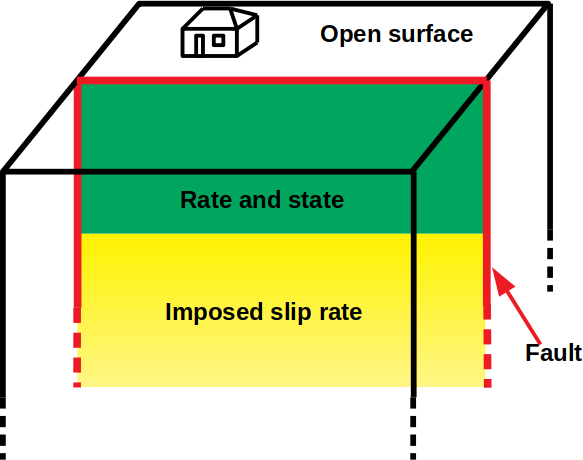
\includegraphics[width=0.3\textwidth]{images/generalSEASModel.png}
	\label{fig:general3DSEASModel}
	\caption{General setup of the SEAS model. Up to a depth $W=24$km, the slip is calculated with rate-and-state friction and everywhere below, the slip is driven by an imposed slip rate}
\end{figure}

To quantify the shift that builds up over time, the slip $S$ is introduced to measure the distance between the displacements $u^+$ and $u^-$ on the two plates that shared a common initial point on the fault. Since the vectors $u$ are 3D displacements but $S$ measures the distance on the 2D fault, the matrix $\mathbf{T}$ is needed  in \autoref{eq:DefinitionSlipAndSlipRate} to extract the tangential components. The normal vector $n$ of the fault surface points from "-" to "+". As a direct consequence of the slip, the slip rate $V$ describes the relative velocity between the plates.
\begin{align}
	\label{eq:DefinitionSlipAndSlipRate}
	S &= \mathbf{T}\left(u^- - u^+\right) \\
	V &= \dv{S}{t}
\end{align}
At the fault, the normal stress $\sigma_n = n_i\bm{\upsigma}_{ij}n_j$ induces, together with some friction coefficient $f$, the fault strength $\tau_S$. In general, a friction law defines a force in opposite direction to the velocity, and in this particular case, the force has a magnitude $\tau_S$. To preserve the force equilibrium along the fault, the internal shear stress $\tau_i=(\delta_{ij}-n_in_j)\bm{\upsigma}_{jk}n_k$ has to cancel out this traction term from the fault. 
\begin{align}
	\tau_S &= \sigma_n f \\
	\tau &= \tau_S\frac{V}{\norm{V}} 
\end{align}
As pointed out by Rice \cite{GeneralSEASSimulations}, the quasi-static model described in \autoref{eq:GeneralElastostaticProblem} cannot handle this velocity-dependent shear traction and needs an additional damping term. For this purpose, we introduce the factor $\eta=\rho c_S/2$ which depends on the density $\rho$ and on the shear wave speed $c_S$. Both parameters are characteristic to the medium and therefore do not change over time. This leads to \autoref{eq:GeneralFrictionLaw}, which will be called \textit{friction law} throughout the thesis. 
\begin{align}
	\label{eq:GeneralFrictionLaw}
	0 &= \norm{\tau} - \sigma_n f - \eta \norm{V}
\end{align}

\subsection{Friction at the fault}
\label{ssec:FrictionLaws}
The coefficient $f$ is calculated by the rate and state friction, which introduces a state variable $\theta$ as a measure for the maturity of contacts, such that the older a fault gets, the stronger it is. A slip over a distance $L$ is sufficient to renew the contact and reset the state variable to 0. This motivates the definition of the ageing law
\begin{equation}
	\dv{\theta}{t} = g^*(\theta, V) = \frac{b}{L}\left(V - V_0e^{\frac{\theta}{b}}\right)
\end{equation} 
to describe the change rate of the state variable. Dieterich \cite{Dieterich79,Dieterich81} and Ruina \cite{Ruina} developed an empirical model to define the friction in function of the absolute slip rate $\norm{V}$ and the state variable $\theta$:
\begin{align}
	\label{eq:GeneralFrictionCoefficient}
	f(V,\theta) &= f_0 + a\ln(\frac{V}{V_0}) + \theta
\end{align}

The constant parameters $f_0$ and $V_0$ stand for the steady-state sliding, that is, if the slip rate reaches $V=V_0$, the state variable vanishes and the friction is equal to $f_0$. In the SEAS model, the parameters $f_0$ and $\theta$ are summed up to form a new state variable $\psi = f_0 +\theta$, which takes the value of $f_0$ at steady-state sliding. Using $\psi$, the ageing law then reads: 

\begin{align}
	\label{eq:GeneralAgeingLaw}
	\dv{\psi}{t} = g(\psi, V) &= \frac{bV_0}{L}\left(e^{\frac{f_0 - \psi}{b}} - \frac{V}{V_0}\right)
\end{align}

The friction coefficient can be further simplified with the summation rule for logarithms because the two terms can be combined in a single logarithm $a\ln(\frac{V}{V_0}e^{\frac{\psi}{a}})$. For very small values of $V$, the logarithm might fail, and a standard remedy \cite{Lapusta} is to replace it with the inverse hyperbolic sine function:

\begin{align}
\label{eq:SEASFrictionCoefficient}
	f(V, \psi) &= a\cdot \text{arsinh}\left(\frac{V}{2V_0}e^{\frac{\psi}{a}}\right)
\end{align}

Indeed, for non-zero slip rates, the term in the logarithm is quite large. In the definition $\text{arsinh} = \text{ln}\left(x + \sqrt{x^2+1}\right)$, the term $+1$ can then be neglected, and the above approximation arises. \\

The parameters $a$ and $b$ describe the material strength under velocity weakening and strengthening and are defined empirically from the experiment in \autoref{fig:DependencyParametersAandB}. The value for $b=0.015$ is chosen constant, and $a$ takes the value $a_0=0.010$ until a depth $h=3$km, it then increases linearly until $a_{max}=0.025$ at a depth $H=15$km, where it remains constant for greater depths. 

\begin{figure}[H]
	\centering
	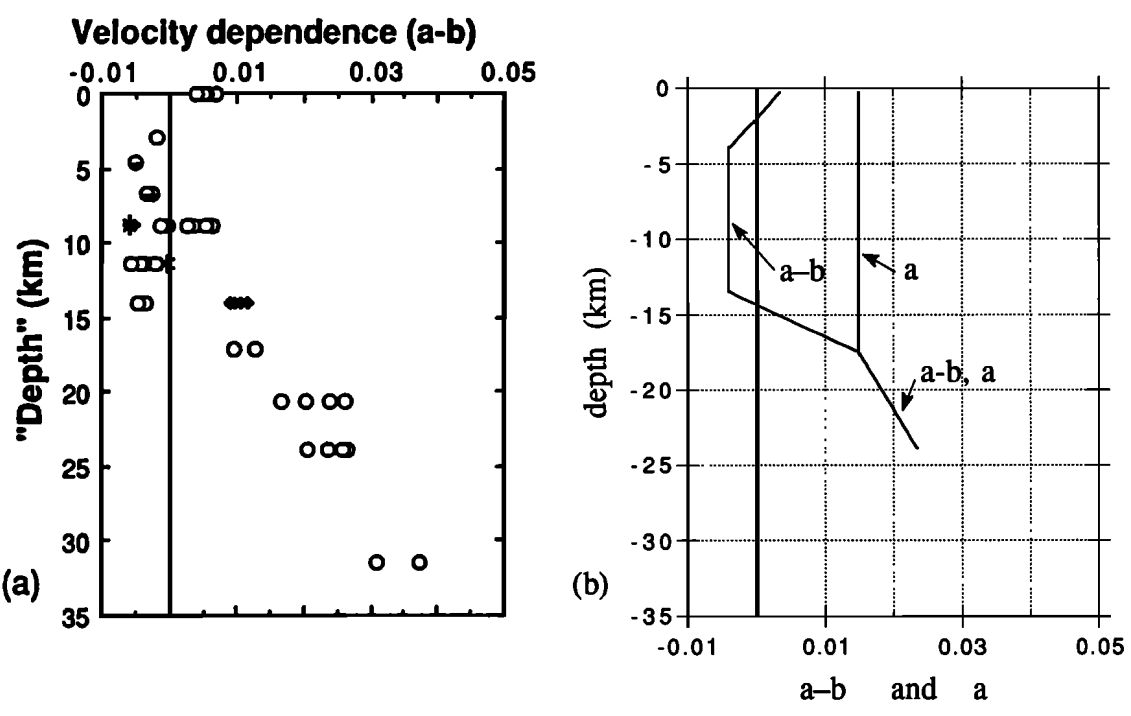
\includegraphics[width=0.7\textwidth]{images/ParametersAandBExperimental.png}
	\caption{Experimental data for granite under hydrothermal conditions on velocity weakening/strengthening in (a) and simplified model for $a$ and $b$ as used in SEAS in (b). Figure taken from \cite{GeneralSEASSimulations}}
	\label{fig:DependencyParametersAandB}
\end{figure}




\section{Differential Algebraic Equations (DAE)}
\label{sec:Theory_DAE}

All in all, the SEAS problem can be resumed to a first order differential algebraic equation (DAE):
\begin{align}
	\label{eq:GeneralSEASDAE}
	\begin{cases}
		\dv{S}{t} = V  & \text{(Slip rate)} \\
		\dv{\psi}{t} = G(\psi, \norm{V}) = \frac{bV_0}{L}\left(e^{\frac{f_0 - \psi}{b}} - \frac{\norm{V}}{V_0}\right) & \text{(Ageing law)} \\
		\;\,\ 0 = F(S,\psi,V) = \norm{\tau(S)} - a \sigma_n(S) \text{arsinh}\left(\frac{\norm{V}}{2V_0}e^{\frac{\psi}{a}}\right) - \eta \norm{V} & \text{(Friction law)}
	\end{cases}	
\end{align}
In general, DAEs differ from ODEs by the fact that the right-hand side of time derivatives cannot be calculated directly and require solving an algebraic equation first. In our case, the slip rate $V$ is needed to evaluate the terms $\dv{S}{t}$ and $\dv{\psi}{t}$ but is not available from the solution vector. \\
From theory, the current problem is a semi-explicit DAE of index 1 \cite[p. 168]{DAETheory}, because $F$ is solvable for $V$. Furthermore, the Jacobian $\pdv{F}{V}$ is invertible as it will be shown in \autoref{sssec:Jacobian_ODE}, so the implicit function theorem can be applied and states that there exists a continuously differentiable expression for $V(S,\psi)$ such that the algebraic condition $F(S,\psi,V(S,\psi))=0$ is fulfilled. \\
For this problem, there exist therefore essentially two approaches: either $V$ is iteratively calculated at each evaluation of the right-hand side of the time derivatives or $V$ is added as an additional component to the solution vector when implicit time integration methods are used. Both approaches, in addition to two others, are investigated in detail in \autoref{chap:44rmulations4SEAS}. \\


\section{Time-adaptive time integration methods}
\label{sec:Theory_TimeIntegration}
Earthquake simulations represent events that occur at several time scales. In the aseismic slip phase, timesteps of the order $h=10^6$s are sufficient whereas, during the earthquake, the rapid changes require timestep sizes as small as $h=10^{-3}$s. To adapt the timestep, an estimate of the local truncation error is needed which indicates whether the stepsize should be increased or decreased. This section presents two families of time integrators, explicit Runge-Kutta and implicit BDF schemes, that come along with such an estimate.

\subsection{Explicit RK methods}
The Runge-Kutta methods are a class of one step method, which calculate the solutions at $s$ intermediate stages to obtain the next timestep. We will only consider the explicit, time-adaptive RK methods. For a general ODE $\dot{x} = \phi(t,x)$ and a stepsize $h$, the next solution $x_{n+1}$ is calculated from the current solution $x_n$ as: 
\begin{equation}
	x_{n+1}	= x_n + h\sum_{i=1}^{s}b_ik_i
\end{equation}
The terms $k_i$ stand for the evaluation of the right-hand side at the different stages and are calculated iteratively as:
\begin{align}
	k_i = \phi\left(t_n + c_ih, x_n + h\sum_{j=1}^{i-1}a_{ij}k_j\right)
\end{align}
For adaptive time-stepping, an estimate of the local truncation error is needed in addition. It is obtained by: 
\begin{equation}
	\varepsilon	= h\sum_{i=1}^{s}(b_i - \bar{b}_i)k_i
\end{equation}
The coefficients $\bar{b}_i$ usually stand for another RK scheme of different order. All coefficients are commonly represented in a Butcher tableau, sketched below.
\begin{center}
\begin{tabular}{c | c c c c c }
	$0$ & & & & & \\
	$c_2$ & $a_{21}$ & & & & \\
	$c_3$ & $a_{31}$ & $a_{32}$ & & & \\  
	$\vdots$ & & & $\ddots$ & & \\
	$c_s$ & $a_{s1}$ & $a_{s2}$ & $\cdots$ & $a_{s,s-1}$ & \\ \hline
	& $b_1$ & $b_2$ & $\cdots$ & $b_{s-1}$ & $b_s$ \\ 
	& $\bar{b}_1$ & $\bar{b}_2$ & $\cdots$ & $\bar{b}_{s-1}$ & $\bar{b}_s$ 
\end{tabular}
\end{center}

An overview of the Butcher tableaus used in this thesis can be found in \autoref{apx:ButcherTableaus}.

\subsection{Implicit BDF methods}
Implicit methods are well-suited for solving stiff problems and allow for higher timesteps than explicit methods. Instead of evaluating the time-derivative in the right-hand side of an ODE for a known solution $\psi_n$, it is evaluated at the next timestep with $\psi_{n+1}$, which is not known. This requires solving an algebraic equation at each timestep without an analytic expression at hand for it. BDF (Backward Differentiation Formula) methods offer a convenient framework for implicit methods up to the order $p=6$. They are multi-step methods, where a method of order $p$ requires the solutions at the $p$ previous timesteps.  \\
A general description of the time-adaptive BDF coefficients can be obtained with the derivatives of the Lagrange interpolation polynomial. If one has a BDF method of order $k$, the coefficients $\alpha_{n+i}$ in front of the previous $k$ solutions are needed to calculate the new solution $\psi_{n+k}$.
\begin{equation}
	\sum_{i=0}^{k}\alpha_{n+i}\psi_{n+i} = f(\psi_{n+k},V_{n+k}) \approx \dot{\psi}_{n+k}
\end{equation} 

To approximate the time derivative $\dot{\psi}_{n+k}$ at the new solution, one could find the polynomial $L(t)$ that interpolates all points $(t_{n+i}, \psi_{n+i})$ and calculate its derivative at the last point $t_{n+k}$. This polynomial $L(t)$ is exactly the Lagrangian interpolation polynomial, calculated as:
\begin{equation}
	L(t) = \sum_{i=0}^{k}\psi_{n+i}\ell_i(t) \qquad\text{with}\qquad \ell_i(t) = \prod_{\substack{0\le j\le k \\j \ne i}}\frac{t-t_{n+j}}{t_{n+i}-t_{n+j}}
\end{equation}

We want to express the derivative $\dot{L}(t)$ at the specific time $t=t_{n+k}$, so that we can approximate $\dot{\psi}_{n+k} \approx \dot{L}(t_{n+k})$ For that, we first need the derivatives of the Lagrange basis polynomials $\dot{\ell}_i(t)$. Because of $\dot{L}(t_{n+k}) = \sum_{i=0}^{k}\dot{\ell}_i(t_{n+k})\psi_{n+k}$, it can be seen that if we evaluate $\dot{\ell}_i(t)$ at the time $t=t_{n+k}$, we obtain exactly the wanted coefficients $\alpha_{n+i}$. The basis polynomials can be calculated with the product rule:
\begin{equation}
	\alpha_{n+i} := \dot{\ell}_i(t_{n+k}) = \sum_{\substack{0\le m\le k \\m \ne i}}\left[\frac{1}{t_{n+i}-t_{n+m}}\prod_{\substack{0\le j\le k \\j \ne i,m}}\frac{t_{n+k}-t_{n+j}}{t_{n+i}-t_{n+j}}\right]
\end{equation}
Alternatively, the time-adaptive BDF coefficients can be derived from Taylor expansions, as described in \autoref{apx:BDF_derivation_Taylor} for the first three schemes.

\subsubsection{Error estimate with an embedded higher-order BDF scheme}
\label{sssec:errorEstimateBDFEmbeddedScheme}
To evaluate the local truncation error at a given timestep, a similar approach as for the time-adaptive Runge-Kutta can be used. If a scheme of order $k$ is used, it involves solving the system a second time with order $k+1$. The error estimate is then the norm of the difference between the two calculated solutions. An obvious drawback of this method is the high computational costs since the evaluation of the error estimate is as expensive as calculating the solution at the next timestep and requires evaluating the right-hand side of the ODE several times, which might be an expensive operation. Another limitation of this method is that the 6th order BDF scheme cannot be used for the time integration, since it implies calculating a 7th order solution for the error estimate, which is not possible because the BDF method is only stable up to the order $k=6$. 

\subsubsection{Error estimate with Lagrange polynomials}
\label{sssec:errorEstimateBDFLagrange}
With the derivatives of the Lagrangian polynomial, a new possibility to estimate the error is available. Once the solution $\psi_{n+k}$ is found, the derivative $\dot{\psi}_{n+k}$ is once approximated with the last $k$ solutions, which gives the coefficients $\alpha_i$, and once with the last $k+1$ solutions, which gives the coefficients $\beta_i$. Now, assume that the $k$th-order approximate results in a perturbed $\dot{\psi}'_{n+k}$ and the $(k+1)$th-order approximates the exact $\dot{\psi}_{n+k}$. We have:
\begin{equation}
	\sum_{i=0}^{k}\alpha_{n+i}\psi_{n+i} = \dot{\psi}'_{n+k} \qquad \text{and}\qquad \sum_{i=-1}^{k}\beta_{n+i}\psi_{n+i} = \dot{\psi}_{n+k} \\
\end{equation}
We now want to find the perturbation $\epsilon$ between the different approximations $\dot{\psi}_{n+k}$ and $\dot{\psi}'_{n+k}$. We get:
\begin{align}
	\sum_{i=0}^{k-1}\alpha_{n+i}\psi_{n+i} + \alpha_{n+k}(\psi_{n+k} + \epsilon) &= \sum_{i=-1}^{k}\beta_{n+i}\psi_{n+i} \nonumber \\ 
	\Leftrightarrow
	\epsilon &= \frac{1}{\alpha_{n+k}}\left(\beta_{n-1}\psi_{n-1} + \sum_{i=0}^{k}(\beta_{n+i}-\alpha_{n+i})\psi_{n+i}\right)
\end{align}
This expression for $\epsilon$ can be used as an estimate for the local truncation error instead of calculating the difference to a higher-order BDF method. The main advantage is that the nonlinear system does not need to be solved twice in one timestep.

\subsection{The PETSc library for time integration}
The Portable, Extensible Toolkit for Scientific Computation (PETSc) \cite{PETSc} offers a convenient framework to efficiently perform many numerical calculations. To perform the previously mentioned RK and BDF methods, the TS component is particularly suitable, as it offers a broad range of Runge-Kutta schemes and all BDF methods of order 1 to 6. It estimates the local truncation error with respectively the embedded RK method and the derivatives of Lagrange polynomials for BDF methods. In addition, TS comes along with a stepsize controller so that the entire adaptive time integration is handled by PETSc. \\

In addition to the TS environment, PETSc routines for vector and matrix operations were used. Furthermore, direct and iterative solvers for linear systems from the KSP and PC components were used in the implementation of the Newton iteration.

\section{Physically motivated time-stepping}
\label{sec:Theory_PhysicalTimeStepping}

Lapusta et al. \cite{Lapusta} proposed a strategy to select the timestep size $h$ depending on the current state of the field variables. It is based on two criteria: first, slow slip rates should allow for large $h$, and second, the relative displacement in each timestep should be small compared to the characteristic slip evolution distance $L$. Together with the local slip rate $V_i$ and a cell parameter $\xi_i$, $h$ can be defined as:
\begin{equation}
	h = \min_i\left[\xi_i L_i / V_i \right]
\end{equation}
The parameter $\xi_i$ depends on the time integration method, the space discretization of the domain, the environment slip rate and the stress gradient and is essentially chosen such that a perturbation at a single node always dies away. Additionally, $\xi_i$ has to be smaller than $1/2$, to avoid that within a timestep, a cell is displaced by more than half the characteristic slip distance $L_i$. \\
This approach is probably fruitful and should always be kept in mind. However, it relies on a highly simplified stability analysis of the problem and this thesis does not investigate it further. Instead, timesteps are only defined through the error estimates of the numerical schemes and are thus not only constrained by physical quantities. Moreover, the divergence issues addressed to define the parameter $\xi_i$ only apply to explicit time integrators with restricted numerical stability and do not pose any problems for implicit methods, whose convergence conditions are much less restrictive.